\documentclass[a4paper,11pt]{book}
\usepackage{lmodern}
\usepackage{amssymb,amsmath}
\usepackage{ifxetex,ifluatex}
\usepackage{fixltx2e} % provides \textsubscript
\ifnum 0\ifxetex 1\fi\ifluatex 1\fi=0 % if pdftex
  \usepackage[T1]{fontenc}
  \usepackage[utf8]{inputenc}
\else % if luatex or xelatex
  \ifxetex
    \usepackage{mathspec}
  \else
    \usepackage{fontspec}
  \fi
  \defaultfontfeatures{Ligatures=TeX,Scale=MatchLowercase}
\fi
% use upquote if available, for straight quotes in verbatim environments
\IfFileExists{upquote.sty}{\usepackage{upquote}}{}
% use microtype if available
\IfFileExists{microtype.sty}{%
\usepackage[]{microtype}
\UseMicrotypeSet[protrusion]{basicmath} % disable protrusion for tt fonts
}{}

\usepackage[colorinlistoftodos]{todonotes}
\newcommand{\mtodo}{\todo[inline]}

\PassOptionsToPackage{hyphens}{url} % url is loaded by hyperref
\usepackage[unicode=true]{hyperref}
\hypersetup{pdfborder={0 0 0},
            breaklinks=true}
\urlstyle{same}  % don't use monospace font for urls
\usepackage{graphicx,grffile}
\makeatletter
\def\maxwidth{\ifdim\Gin@nat@width>\linewidth\linewidth\else\Gin@nat@width\fi}
\def\maxheight{\ifdim\Gin@nat@height>\textheight\textheight\else\Gin@nat@height\fi}
\makeatother
% Scale images if necessary, so that they will not overflow the page
% margins by default, and it is still possible to overwrite the defaults
% using explicit options in \includegraphics[width, height, ...]{}
\setkeys{Gin}{width=\maxwidth,height=\maxheight,keepaspectratio}
\IfFileExists{parskip.sty}{%
\usepackage{parskip}
}{% else
\setlength{\parindent}{0pt}
\setlength{\parskip}{6pt plus 2pt minus 1pt}
}

\setlength{\oddsidemargin}{0mm}
\setlength{\evensidemargin}{-14mm}
\setlength{\marginparwidth}{0cm}
\setlength{\marginparsep}{0cm}
\setlength{\topmargin}{2mm}
\setlength{\textwidth}{168mm}
\setlength{\textheight}{240mm}
\setlength{\footskip}{10mm}

\setlength{\emergencystretch}{3em}  % prevent overfull lines
\providecommand{\tightlist}{%
  \setlength{\itemsep}{0pt}\setlength{\parskip}{0pt}}

%\setcounter{secnumdepth}{0}
% Redefines (sub)paragraphs to behave more like sections
\ifx\paragraph\undefined\else
\let\oldparagraph\paragraph
\renewcommand{\paragraph}[1]{\oldparagraph{#1}\mbox{}}
\fi
\ifx\subparagraph\undefined\else
\let\oldsubparagraph\subparagraph
\renewcommand{\subparagraph}[1]{\oldsubparagraph{#1}\mbox{}}
\fi

\usepackage{color}
\usepackage{fancyvrb}
\newcommand{\VerbBar}{|}
\newcommand{\VERB}{\Verb[commandchars=\\\{\}]}
\DefineVerbatimEnvironment{Highlighting}{Verbatim}{commandchars=\\\{\}}
% Add ',fontsize=\small' for more characters per line
\newenvironment{Shaded}{}{}
\newcommand{\KeywordTok}[1]{\textcolor[rgb]{0.00,0.44,0.13}{\textbf{#1}}}
\newcommand{\DataTypeTok}[1]{\textcolor[rgb]{0.56,0.13,0.00}{#1}}
\newcommand{\DecValTok}[1]{\textcolor[rgb]{0.25,0.63,0.44}{#1}}
\newcommand{\BaseNTok}[1]{\textcolor[rgb]{0.25,0.63,0.44}{#1}}
\newcommand{\FloatTok}[1]{\textcolor[rgb]{0.25,0.63,0.44}{#1}}
\newcommand{\ConstantTok}[1]{\textcolor[rgb]{0.53,0.00,0.00}{#1}}
\newcommand{\CharTok}[1]{\textcolor[rgb]{0.25,0.44,0.63}{#1}}
\newcommand{\SpecialCharTok}[1]{\textcolor[rgb]{0.25,0.44,0.63}{#1}}
\newcommand{\StringTok}[1]{\textcolor[rgb]{0.25,0.44,0.63}{#1}}
\newcommand{\VerbatimStringTok}[1]{\textcolor[rgb]{0.25,0.44,0.63}{#1}}
\newcommand{\SpecialStringTok}[1]{\textcolor[rgb]{0.73,0.40,0.53}{#1}}
\newcommand{\ImportTok}[1]{#1}
\newcommand{\CommentTok}[1]{\textcolor[rgb]{0.38,0.63,0.69}{\textit{#1}}}
\newcommand{\DocumentationTok}[1]{\textcolor[rgb]{0.73,0.13,0.13}{\textit{#1}}}
\newcommand{\AnnotationTok}[1]{\textcolor[rgb]{0.38,0.63,0.69}{\textbf{\textit{#1}}}}
\newcommand{\CommentVarTok}[1]{\textcolor[rgb]{0.38,0.63,0.69}{\textbf{\textit{#1}}}}
\newcommand{\OtherTok}[1]{\textcolor[rgb]{0.00,0.44,0.13}{#1}}
\newcommand{\FunctionTok}[1]{\textcolor[rgb]{0.02,0.16,0.49}{#1}}
\newcommand{\VariableTok}[1]{\textcolor[rgb]{0.10,0.09,0.49}{#1}}
\newcommand{\ControlFlowTok}[1]{\textcolor[rgb]{0.00,0.44,0.13}{\textbf{#1}}}
\newcommand{\OperatorTok}[1]{\textcolor[rgb]{0.40,0.40,0.40}{#1}}
\newcommand{\BuiltInTok}[1]{#1}
\newcommand{\ExtensionTok}[1]{#1}
\newcommand{\PreprocessorTok}[1]{\textcolor[rgb]{0.74,0.48,0.00}{#1}}
\newcommand{\AttributeTok}[1]{\textcolor[rgb]{0.49,0.56,0.16}{#1}}
\newcommand{\RegionMarkerTok}[1]{#1}
\newcommand{\InformationTok}[1]{\textcolor[rgb]{0.38,0.63,0.69}{\textbf{\textit{#1}}}}
\newcommand{\WarningTok}[1]{\textcolor[rgb]{0.38,0.63,0.69}{\textbf{\textit{#1}}}}
\newcommand{\AlertTok}[1]{\textcolor[rgb]{1.00,0.00,0.00}{\textbf{#1}}}
\newcommand{\ErrorTok}[1]{\textcolor[rgb]{1.00,0.00,0.00}{\textbf{#1}}}
\newcommand{\NormalTok}[1]{#1}

% set default figure placement to htbp
\makeatletter
\def\fps@figure{htbp}
\makeatother

\newcommand{\code}[1]{\texttt{#1}}

\title{Mutley's Guide To The Wacky Racers, V1E-3}
\author{Michael Hayes and Ben Mitchell}
\date{2021}

\begin{document}
\maketitle

\chapter{Hardware}


\section{Introduction}\label{introduction}

An hour spent checking your schematic will avoid many hours of testing
grief!

\subsection{Recommendations}\label{recommendations}

\begin{enumerate}
\item
  Independently fuse the buck converter and H-bridge. This allows a fuse
  to be removed to isolate part of the circuit when finding a fault,
  such as a short across the power rails.

\item
  Have a zener diode to protect against overvoltage input from a bench
  power supply.

\item
  Have current limiting resistors for all off-board signals.

\item
  Have plenty of testpoints, especially for power supplies and signals.
  You will never have too many!

\item
  Have at least one grunty ground testpoint for attaching a scope ground
  clip.

\item
  Have a dedicated PIO pin to drive a testpoint that you can use to
  trigger an oscilloscope for debugging.

\item
  Have the SAM4S erase pin connected to a test point close to a 3.3 V
  testpoint. This is useful to completely erase the SAM4S flash memory
  when nothing works.
\end{enumerate}

\section{SAM4S MCU}\label{sam4s-mcu}

The SAM4S MCU is overkill for this assignment but is typical of
ARM processors used for bare-metal applications.

\subsection{Power pins}\label{power-pins}

The SAM4S has four grounds. They must all be connected. There are also
seven power pins. These must all be connected since they power different
parts of the chip. Note, some pins require 3.3 V while others require
1.2 V. The 1.2 V is generated by an internal voltage regulator.

\subsection{Peripheral pins}\label{peripheral-pins}

\textbf{Many of the peripheral pins are dedicated and cannot be
reassigned in software}, e.g., SPI, TWI, and USB pins. Note, there are
restrictions on the PWM pins.

By default the \pin{PB4} and \pin{PB5} pins are configured for the JTAG debugger.
These can be used for general PIO after setting an internal bit.  See
\protect\hyperref[disabling-jtag-pins]{disabling JTAG pins}.

The logic levels are set by the voltage on the VDDIO pin (usually
3.3\,V).  \pin{PA12}--\pin{PA14} and \pin{PA26}--\pin{PA31} can sink/source
4\,mA.  The USB pins (\pin{PB10}--\pin{PB11}) can sink/source 30\,mA.  The
rest can only sink/source 2\,mA of current


\subsection{USART/UART}\label{usartuart}

The SAM4S has two USARTs and two UARTs. The USARTs can emulate a
UART, have hardware flow control, and have a better driver so they are
recommended if you need a UART interface.


\subsection{PWM}\label{pwm}

The SAM4S can generate four independent PWM signals. There are
restrictions on which SAM4S pins they come out on. Note, the PWMLx and
PWMHx signals are complementary.

\subsection{TWI}\label{twi}

The SAM4S has two TWI peripherals (that can act as a master and
a slave) with dedicated TWD and TWCK pins. External pull-up resistors
are required.  TWI1 shares pins with JTAG; you will need to disable
JTAG in software.

\subsection{SPI}\label{spi}

The SAM4S has a single SPI peripheral with dedicated SCK, MISO,
and MOSI pins. Any PIO pin can be used for the chip
select\footnote{For high speed operation, you should use on of the
  dedicated chip select pins.}.

\subsection{ADC}\label{adc}

The SAM4S has a single ADC with a multiplexer to select one of a
number of analogue inputs.  It can sample at 1\,MHz.

\subsection{USB}\label{usb}

The SAM4S has a single USB peripheral connected to the DDP and DDM
pins. 27 ohm series termination resistors are required, placed close to
the SAM4S.

\section{Other chips}\label{other-chips}

\subsection{DRV8833 dual H-bridge}\label{drv8833-dual-h-bridge}

The capacitor connected to the bootstrap pin must be rated for 16 V. The
datasheet recommends an X7R dielectric.

If you want control over fast decay and slow decay in both forward and
reverse you will need four PWM signals. The SAM4S can provide four
independent PWM signals but be careful that PWMxH and PWMxL are driven
with the same PWM signal but are complementary.

You can drive the H-bridge with only two PWM signals but you will have
fast decay in one direction and slow decay in the other. It appears that
fast decay is better at slow speeds since the motor heats less.

\subsection{NRF24L01+ radio}\label{nrf24l01-radio}

This operates around 2.4 GHz and has 128 programmable channels, each of
1 MHz. A 5 byte address is appended to the start of each transmission
and the receiver will only respond when the address matches.

The radio interfaces to the SAM4S using the SPI bus. The IRQ
pin is driven low to indicate a packet has been received.

A well filtered power supply is critical otherwise the range will be
limited on reception. Preferably, the device should have its own 3V3
regulator with a low-pass RC filter comprised of a series resistor and
large capacitor (say 22 uF) or a low-pass LC filter made with a ferrite
bead and capacitor.

\subsection{MPU9250 IMU}\label{mpu9250-imu}

This contains a three axis accelerometer, a three axis gyroscope, and a
three axis magnetometer. It appears that the magnetometer has been
bolted on to the accelerometers/gyroscopes and requires more hoop
jumping in software to make it work.

It has two different I2C addresses (0X68 and OX69) depending on
the state of the AD0 pin.


\subsection{Voltage regulators}\label{voltage-regulators}

There are many flavours of \wikiref{voltage_regulators}{voltage regulator}.
Some are better for digital applications, some are better for analogue
applications, some are better for low power applications, etc.

If you are using a voltage regulator with an enable pin, do not forget
to allow for the time for the output voltage to ramp up. This can be
tens of milliseconds depending on the capacitive load and current draw.

Note, some regulators have pins that you must not connect. Some have
multiple pins for the same purpose; these must all be connected.

\section{PCB recommendations}\label{pcb-recommendations}

\subsection{Placement}\label{placement}

\begin{enumerate}
\item
  Keep small signal analogue components (radio) well away from digital
  electronics and power electronics.
\item
  Place local decoupling capacitors to minimise the loop area.
\item
  Keep the crystal close to the MCU.
\item
  Place switches so they can be pushed.
\item
  Place LEDs so they can be seen.
\item
  Place USB connector so it can be connected to.
\item
  Place connectors on edge with wires going away from the board.
\end{enumerate}

\subsection{Check list}\label{check-list}

\begin{enumerate}
\item
  No planes under the radio antenna.
\item
  The SPI signals for the radio are connected to the correct MCU pins.
\item
  The PWM signals for the motor are connected to the correct MCU pins.
  Note, the PWMLx and PWMHx pins are complementary and cannot be driven
  independently.
\item
  All the MCU VDD pins need to be powered.
\item
  All the MCU GND pins need to be powered.
\item
  Avoid connecting to \pin{PB4} and \pin{PB5} (say for TWI1).  If you do you will need to disable JTAG.
\end{enumerate}


\chapter{Software}

\section{Preparation}
\label{preparation}

Do not underestimate the effort required to flash your first LED. You
require:

\begin{itemize}
\item
  A computer with \program{git} installed and a useful shell program such as
  \program{bash}. UC has a \href{http://ucmirror.canterbury.ac.nz/}{mirror}
  for a variety of Linux distributions; we recommend Ubuntu or Mint.
\item
  A working ARM toolchain (arm-none-eabi-gcc/g++ version 4.9.3 or newer).
\item
  \program{OpenOCD} V0.8.0 or later.
\item
  An ST-link programmer and 10-wire ribbon cable for programming. You
  can get the adaptor from Scott Lloyd in the SMT lab. You will need
  to make your own cable (For a grey ribbon cable, align the red
  stripe with the small arrow denoting pin 1 on the connector. For a
  rainbow ribbon cable, connect the brown wire to pin 1.). There are
  two variants of the ST-link programmer with \textbf{different
    pinouts} so you may need to customise your programming cable.
\item
  Plenty of gumption.
\end{itemize}

\subsection{Toolchain}
\label{toolchain}

The required software is installed on computers in the ESL and
CAE. It should run under both Linux and Windows. If there is a
problem ask the technical staff.

If you are working from a personal Linux computer make sure to update
your machine to the latest software versions. This is particularly
important for the ARM toolchain (arm-none-eabi-gcc/g++) which should be
at version 4.9.3 or newer. You can do this with the following command
for an Ubuntu or Mint distribution:

\begin{minted}{bash}
$ sudo apt update && sudo apt upgrade}
\end{minted}

For MacOS machines that have \href{https://brew.sh}{homebrew} installed,
you can use the following command:

\begin{minted}{bash}
$ brew install openocd git}
$ brew cask install gcc-arm-embedded}
\end{minted}

\subsection{Project forking}
\label{project-forking}

The example software is hosted on the eng-git \program{Git} server at
\href{https://eng-git.canterbury.ac.nz/wacky-racers/wacky-racers-2021}{\url{https://eng-git.canterbury.ac.nz/wacky-racers/wacky-racers-2021}}.
Your group leader should have forked this template project. This creates
your own group copy of the project on the eng-git server that you can
modify, add members, etc. To fork the project:

\begin{enumerate}
\item
  Go to
  \href{https://eng-git.canterbury.ac.nz/wacky-racers/wacky-racers-2021}{\url{https://eng-git.canterbury.ac.nz/wacky-racers/wacky-racers-2021}}.
\item
  Click the `Fork' button. This will create a copy of the main repository
  for the project.
\item
  Click on the `Settings' menu then click the `Expand' button for
  `Sharing and permissions'. Change `Project Visibility' to `Private'.
\item
  Click on the `Members' menu and add group members as Developers.
\end{enumerate}

\subsection{Project cloning}
\label{project-cloning}

Once your project has been forked from the template project, each group
member needs to clone it. This makes a local copy of your project on
your computer. 

If you are using an ECE computer, it is advised that you clone the
project on to a removable USB flash drive. This will make git operations
and compilation a 100 times faster than using the networked file system.

There are two ways to clone the project. If you are impatient and do not
mind having to enter a username and password for every git pull and push
operation use:
%
\begin{minted}[breaklines]{bash}
$ git clone https://eng-git.canterbury.ac.nz/groupleader-userid/wacky-racers-2021.git wacky-racers
\end{minted}

Otherwise, set up \program{ssh-keys} and use:
%
\begin{minted}[breaklines]{bash}
$ git clone git@eng-git.canterbury.ac.nz:groupleader-userid/wacky-racers-2021.git wacky-racers
\end{minted}

You can several different cloned copies of your project in different
directories. Sometimes if you feel that the world, and \program{git} in
particular, is against you, clone a new copy, using:


\begin{minted}[breaklines]{bash}
$ git clone https://eng-git.canterbury.ac.nz/groupleader-userid/wacky-racers-2021.git wacky-racers-new
\end{minted}

\subsection{Configuration}
\label{configuration}

Each board has different PIO definitions and requires its own
configuration information. The \wfile{boards}
directory contains a number of configurations; one for the hat and racer
boards. Each configuration directory contains three files:

\begin{itemize}
\item
  \file{board.mk} is a makefile fragment that specifies the MCU model,
  optimisation level, etc.
\item
  \file{target.h} is a C header file that defines the PIO pins and
  clock speeds.
\item
  \file{config.h} is a C header file that wraps target.h. It's purpose
  is for porting to different compilers.
\end{itemize}

\textbf{You will need to edit the target.h file for your board} and set
the definitions appropriate for your hardware. Here's an excerpt from
\file{target.h} for a hat board:

\begin{minted}{C}
/* USB  */
#define USB_VBUS_PIO PA5_PIO

/* ADC  */
#define ADC_BATTERY PB3_PIO
#define ADC_JOYSTICK_X PB2_PIO
#define ADC_JOYSTICK_Y PB1_PIO

/* IMU  */
#define IMU_INT_PIO PA0_PIO

/* LEDs  */
#define LED1_PIO PA20_PIO
#define LED2_PIO PA23_PIO
\end{minted}

\section{First program}
\label{first-program}

Your first program to test your board should only flash an LED (the
hello world equivalent for embedded systems). The key to testing new
hardware is to have many programs that only do one simple task each.

\subsection{OpenOCD}
\label{openocd}

\program{OpenOCD} is used to program the SAM4S. For this assignment,
we are using a ST-link programmer to connect to the SAM4S using serial
wire debug (SWD). This connects to your board with a 10-wire ribbon
cable and an IDC connector.

\begin{enumerate}
\item
  Before you start, disconnect the battery and other cables from your
  PCB.
\item
  Connect a 10-wire ribbon cable from the ST-link programmer to the
  programming header on your PCB. This will provide 3.3 V to your
  board so your green power LED should light.
\item
  Open a \textbf{new terminal window} and start \program{OpenOCD}.
\end{enumerate}

\begin{minted}{bash}
$ cd wacky-racers
$ openocd -f src/mat91lib/sam4s/scripts/sam4s_stlink.cfg
\end{minted}

All going well, the last line output from \program{OpenOCD} should be:

\begin{verbatim}
Info : sam4.cpu: hardware has 6 breakpoints, 4 watchpoints
\end{verbatim}

Congrats if you get this! It means you have correctly soldered your
SAM4S. If not, do not despair and do not remove your SAM4S. Instead,
see \protect\hyperref[troubleshooting]{troubleshooting}.


\subsection{LED flash program}
\label{led-flash-program}

For your first program, use
\wfile{test-apps/ledflash1/ledflash1.c}. The macros
\code{LED1\_PIO} and \code{LED2\_PIO} need to be defined in
\file{target.h} (see
\protect\hyperref[configuration]{configuration}). If your LEDs are
active high, replace 1 with 0 in the LED config structures.

\inputminted{C}{../../src/test-apps/ledflash1/ledflash1.c}

\subsection{Compilation}
\label{compilation}

Due to the many files required, compilation is performed using
makefiles.

The demo test programs are generic and you need to specify which board
you are compiling them for. The board configuration file can be chosen
dynamically by defining the environment variable \code{BOARD}. For
example:
%
\begin{minted}{bash}
$ cd src/test-apps/ledflash1
$ BOARD=racer make
\end{minted}

If all goes well, you should see at the end:
%
\begin{verbatim}
   text    data     bss     dec     hex filename
  19432    2420    2732   24584    6008 ledflash1.bin
\end{verbatim}

To avoid having to specify the environment variable \code{BOARD}, you
can define it for the rest of your session using:
%
\begin{minted}{bash}
$ export BOARD=racer
\end{minted}
%
and then just use:
%
\begin{minted}{bash}
$ make
\end{minted}

Note, if you compile with the \code{BOARD} environment variable set incorrectly, use:
%
\begin{minted}{bash}
$ make clean
$ make  
\end{minted}
%
to delete all the object files and rebuild.


\subsection{Booting from flash memory}
\label{booting-from-flash-memory}

By default the SAM4S runs a bootloader program stored in ROM. The SAM4S
needs to be configured to run your application in flash memory.

If \program{OpenOCD} is running you can do this with:

\begin{minted}{bash}
$ make bootflash
\end{minted}

Unless you force a complete erasure of the SAM4S flash memory by
connecting the \pin{ERASE} pin to 3.3 V, you will not need to repeat
this command.

\subsection{Programming}
\label{programming}

If \program{OpenOCD} is running you can store your program in the flash
memory of the SAM4S using:

\begin{minted}{bash}
$ make program
\end{minted}

When this finishes, one of your LEDs should flash. If so, congrats! If
not, see \protect\hyperref[troubleshooting]{troubleshooting}.

To reset your SAM4S, you can use:
%
\begin{minted}{bash}
$ make reset
\end{minted}

\section{USB interfacing}
\label{usb-interfacing}

To help debug your programs, it is wise to set up USB CDC. For
example, here's the code for
\wfile{test-apps/usb_serial_test1/usb_serial_test1.c}.

\inputminted{C}{../../src/test-apps/usb_serial_test1/usb_serial_test1.c}

Note, the string \code{"/dev/usb\_tty"} is used to name the USB serial
device on the SAM4S so that it can be used by the C stdio function
\code{freopen}.   

To get this programme to work you need to compile it and program the SAM4S using:

\begin{minted}{bash}
$ cd wacky-racers/src/test-apps/usb_serial_test1
$ make program
\end{minted}

You then need to connect your computer to the USB connector on your PCB.
If you are running Linux, run:
%
\begin{minted}{bash}
$ dmesg
\end{minted}

This should say something like:
%
\begin{verbatim}
Apr 30 11:03:50 thing4 kernel: [52704.481352] usb 2-3.3: New USB device found, idVendor=03eb, idProduct=6202
Apr 30 11:03:50 thing4 kernel: [52704.481357] usb 2-3.3: New USB device strings: Mfr=1, Product=2, SerialNumber=3
Apr 30 11:03:50 thing4 kernel: [52704.482060] cdc_acm 2-3.3:1.0: ttyACM0: USB ACM device
\end{verbatim}

Ignore the errors for now\footnote{They have popped up with new Linux
  kernels and we have yet to determine why.}. If you see
\texttt{ttyACM0:\ USB\ ACM\ device} congrats. If not, see
\href{USB_debugging}{USB debugging}.

You can now run a serial terminal program. For example, on Linux:

\begin{minted}{bash}
$ gtkterm -p /dev/ttyACM0
\end{minted}

All going well, this will repeatedly print 'Hello world'.

If you get an error 'device is busy', it is likely that the ModemManager
program has automatically connected to your device on the sly. This
program should be disabled on the ECE computers. For more about this and
using other operating systems, search for USB CDC on ecewiki.

\section{Test programs}
\label{test-programs}

There are a number of test programs in the directory
\wfile{test-apps}. Where possible these are written to be
independent of the target board using configuration files (see
\protect\hyperref[configuration]{configuration}).

\subsection{PWM test}
\label{pwm-test}

The program \wfile{test-apps/pwm_test2/pwm_test2.c} provides an
example of driving PWM signals. Notes:
%
\begin{enumerate}
\item
  This is for a different H-bridge module that requires two PWM signals
  and forward/reverse signals. You will need to generate four PWM
  signals or be clever with two PWM signals.
\item
  The \code{pwm\_cfg\_t} structure configures the frequency, duty
  cycle and alignment of the output PWM.
\end{enumerate}

The most likely problem is that you have not used a PIO pin that can
be driven as a PWM output. The SAM4S can generate four independent
hardware PWM signals. See \wfile{mat91lib/pwm/pwm.c} for a list of
supported PIO pins. Note, \pin{PA16}, \pin{PA30}, and \pin{PB13} are
different options for PWM2.

To drive the motors you will need to use a bench power supply. Start
with the current limit set at 100\,mA maximum in case there are any
board shorts.  When all is well, you can increase the current limit.

\subsection{IMU test}
\label{imu-test}

The program \wfile{test-apps/imu_test1/imu_test1.c} provides an
example of using the MPU9250 IMU.  All going well, this prints three
16-bit acceleration values per line to USB CDC. Tip your board over,
and the the third (z-axis) value should go negative since this
measures the effect of gravity on a little mass inside the IMU pulling
on a spring.

If you get 'Cannot detect IMU' the main reasons are:

\begin{enumerate}
\item
  You have specified the incorrect address. Use \code{MPU\_0} if the
  AD0 pin is connected to ground otherwise use \code{MPU\_1}.
\item
  You are using TWI1. The \pin{PB4} and \pin{PB5} pins used by TWI1 default to JTAG
  pins. See \protect\hyperref[disabling-jtag-pins]{disabling JTAG pins}.
\item
  You do not have TWI/I2C pull-up resistors connected to 3V3 or the
  wrong resistor values. Use a scope to look at the signals \pin{TWCK/SCL}
  and \pin{TWD/SDA}.
\item
  Check that the auxiliary I2C bus signals are not connected
  (otherwise the magnetometer will not respond).  
\item
  You have a soldering problem. Try pressing on a side of the IMU with a
  fingernail to see if it starts working.
\end{enumerate}

If you reset the SAM4S in the middle of a transaction with the
IMU, the IMU gets confused and holds the \pin{TWD/SDA} line low. This
requires recycling of the power or sending out some dummy clocks on
the \pin{TWCK/SCL} signal.


\subsection{Radio test}
\label{radio-test}

The program \wfile{test-apps/radio_tx_test1/radio_tx_test1.c} provides
an example of using the radio as a transmitter.

The companion program
\wfile{test-apps/radio_rx_test1/radio_rx_test1.c} provides an example
of using the radio as a receiver.

Notes:
%
\begin{enumerate}
\item
  Both programs must use the same RF channel and the same address. Some
  RF channels are better than others since some overlap with WiFi
  and Bluetooth. The address is used to distinguish devices
  operating on the same channel. Note, the transmitter expects an
  acknowledge from a receiver on the same address and channel.
\item
  The radio `write` method blocks waiting for an auto-acknowledgement
  from the receiver device. This acknowledgement is performed in
  hardware. If no acknowledgement is received, it retries for up to 15
  times. The auto-acknowledgement and number of retries can be
  configured in software.
\end{enumerate}

If you cannot communicate between your hat and racer boards, try
communicating with the radio test modules Scott Lloyd has in the SMT
lab.

\section{Your hat/racer program}
\label{your-hatracer-program}

There is skeleton code, see
\wfile{wacky-apps/hat/hat.c} and
\wfile{wacky-apps/racer/racer.c}. We recommend that
build your programs incrementally and that you poll your devices with a
paced loop and not use interrupts. It is a good idea to disable the
watchdog timer until you have robust code.

\begin{minted}{C}
#include <stdio.h>
#include <math.h>
#include "mcu.h"
#include "pacer.h"

// Set to the desired polling rate.
#define PACER_RATE 1000

int
main (void)
{
    // If you are using PB4 or PB5 (say for TWI1) uncomment the next line.
    // mcu_jtag_disable ();    

    pacer_init (PACER_RATE);    
    
    mcu_watchdog_enable ();

    while (1)
    {
        pacer_wait ();

        mcu_watchdog_reset ();

        /* Do your stuff here...  */
        
    }
    
    return 0;
}
\end{minted}

\section{Debugging}
\label{debugging}

If \program{OpenOCD} is running, a running program can be debugged using:

\begin{minted}{bash}
$ make debug
\end{minted}

This starts \program{GDB} and attaches to the target MCU. \program{GDB} is a
command line debugger but there are many GUI programs that will control
it, for example, \program{vscode} and \program{geany} have plugins.

\program{GDB} allows you to inspect the CPU registers, memory, set
breakpoints, set watchpoints, and much more. The only gnarly thing is
that when compiling with optimisation, the compiler may reorder
statements or even remove them. Debugging embedded systems is also made
difficult by the asynchronous nature of I/O.

You can reset your program using the GDB `jump reset` command. However,
this does not reset the peripherals as with a power-on reset.

\section{Howtos}
\label{howtos}

\subsection{Disabling JTAG pins}
\label{disabling-jtag-pins}

By default \pin{PB4} and \pin{PB5} are configured as JTAG pins. You can turn
them into PIO pins or use them for TWI1 using:
%
\begin{minted}{C}
#include "mcu.h"

void main (void)
{
    mcu_jtag_disable ();
}
\end{minted}

\subsection{Watchdog timer}
\label{watchdog-timer}

The watchdog timer is useful for resetting the SAM4S if it hangs in a
loop.  It is disabled by default but can be enabled using:
%
\begin{minted}{C}
#include "mcu.h"

void main (void)
{
    mcu_watchdog_enable ();
   
    while (1)
    {
         /* Do your stuff here.  */

         mcu_watchdog_reset ();
    }
}
\end{minted}

\section{Under the bonnet}
\label{under-the-bonnet}

\file{wackylib} is a library of C files that tries to hide some of the
complexity of the underlying software.

\file{mmculib} is a library of C drivers, mostly for performing high-level I/O.
It is written to be microcontroller neutral.

\file{mat91lib} is a library of C drivers specifically for interfacing
with the peripherals of Atmel AT91 microcontrollers such as the Atmel
SAM4S. It provides the hardware abstraction layer.

The building is controlled by \wfile{mat91lib/mat91lib.mk}. This is a
makefile fragment loaded by \wfile{mmculib/mmculib.mk}.
\file{wacky-reacers/src/mat91lib/mat91lib.mk} loads other makefile fragments for each
peripheral or driver required. It also automatically generates
dependency files for the gazillions of other files that are required to
make things work.

\section{Git}
\label{git}

To properly use git you should commit and push often. The smaller the
changes and the more often you make per commit, the smaller the chance
of the dreaded merge conflict.

\subsection{Git pulling from upstream}
\label{git-pulling-from-upstream}

To be able to get updates if the template project is modified you will
need to:

\begin{minted}{bash}
$ cd wacky-racers 
$ git remote add upstream https://eng-git.canterbury.ac.nz/wacky-racers/wacky-racers-2021.git  
\end{minted}

Again if you do not want to manually enter your password (and have
ssh-keys uploaded) you can use:
%
\begin{minted}[breaklines]{bash}
$ cd wacky-racers 
$ git remote add upstream git@eng-git.canterbury.ac.nz:wacky-racers/wacky-racers-2021.git
\end{minted}

Once you have defined the upstream source, to get the updates from the
main repository use:
%
\begin{minted}{bash}
$ git pull upstream master
\end{minted}

If you enter the wrong URL make a mistake, you can list the remote
servers and delete the dodgy entry using:

\begin{minted}{bash}
$ git remote -v
$ git remote rm upstream
\end{minted}

Note, \textbf{origin} refers to your group project and \textbf{upstream}
refers to the template project that origin was forked from.

\subsection{Git merging}
\label{git-merging}

The bane of all version control programs is dealing with a merge
conflict. You can reduce the chance of this happening by committing and
pushing faster than other people in your group.

If you get a message such as:

\begin{verbatim}
From https://eng-git.canterbury.ac.nz/wacky-racers/wacky-racers-2021
 * branch            master     -> FETCH_HEAD
error: Your local changes to the following files would be overwritten by merge:
    src/test-apps/imu_test1/imu_test1.c
Please, commit your changes or stash them before you can merge.
\end{verbatim}

what you should so is:

\begin{minted}{bash}
$ git stash
$ git pull
$ git stash pop
# You may now have a merge error.  You will now have to edit the offending file, in this case imu_test1.c
# Once the file has been fixed
$ git add src/test-apps/imu_test1/imu_test1.c
$ git commit -m "Fix merge"
\end{minted}

Sometimes when you do a git pull you will be thrown into a text editor
to type a merge comment. The choice of editor is controlled by an
environment variable \code{EDITOR}. On the ECE computers this defaults
to emacs. You can changed this by adding a line such as the following to
the \file{.bash\_profile} file in your home directory.

\begin{minted}{bash}
$ export EDITOR=geany
\end{minted}

By the way, to exit emacs type ctrl-x ctrl-c, to exit vi or vim type \code{:q!}

\textbf{Please do not edit the files in the mat91lib, mmculib, and
wackylib} directories since this can lead to merge problems in the
future. If you find a bug or would like additional functionality let MPH
or one of the TAs know.

\chapter{Troubleshooting}
\label{troubleshooting}

Troubleshooting can be frustrating when you are tired. You need plenty
of gumption and an open mind. Difficult problems are usually a
combination of two or more problems. So \textbf{do not attempt if you
are tired or in a hurry} .

\section{Oscilloscope}
\label{oscilloscope}

The best tool for debugging an embedded system is an oscilloscope.

\begin{enumerate}
\item
  Use x10 probes.
\item
  Use the correct probes for the scope so that they can be automatically
  detected.
\item
  Compensate the probes by clipping to the probe test signal on the
  scope and adjusting the variable capacitor in the probe to ensure a
  square wave without undershoot or overshoot. This is one of the few
  times you are allowed to use the autoscale button!
\end{enumerate}

\subsection{Normal mode}
\label{normal-mode}

This mode is for measuring transient or non-repetitive signals. It will
only refresh the display if a trigger event is detected.

It is useful to increase the \emph{trigger holdoff} to prevent
triggering on multiple edges of a waveform. By default, it is set to a
ridiculously small value.

\subsection{Auto mode}
\label{auto-mode}

This mode is for measuring AC or DC signals. It is like normal mode but
if it does not detect a trigger it will automatically refresh the
display.

\section{SAM4S not detected by OpenOCD}
\label{sam4s-not-detected-by-openocd}

If a program has not been loaded:

\begin{enumerate}
\item
  Check orientation of the SAM4S.
\item
  Check soldering of the SAM4S pins under a microscope. Giving
  each pin a push with a sharp spike can reveal a poorly soldered joint.
\item
  Check 3.3 V and 1.2 V power rails.
\item
  Check the serial wire debug (SWD) signals, see
  \protect\hyperref[debugging]{Debugging serial wire debug (SWD)}.
\end{enumerate}

If a program has been loaded:

\begin{enumerate}
\item
  Check the crystal oscillator, see
  \protect\hyperref[checking-the-crystal-oscillator]{Checking the
  crystal oscillator}.
\item
  Erase the flash memory by connecting the ERASE pin to 3.3 V, re-enable
  booting from flash, and reprogram the SAM4S with an LED flash
  program.
\end{enumerate}

\subsubsection{Debugging serial wire debug (SWD)}
\label{debugging-serial-wire-debug-swd}

\program{OpenOCD} periodically polls to see if the SAM4S is alive.
These occur every 100\,ms.

\begin{figure}
\centering
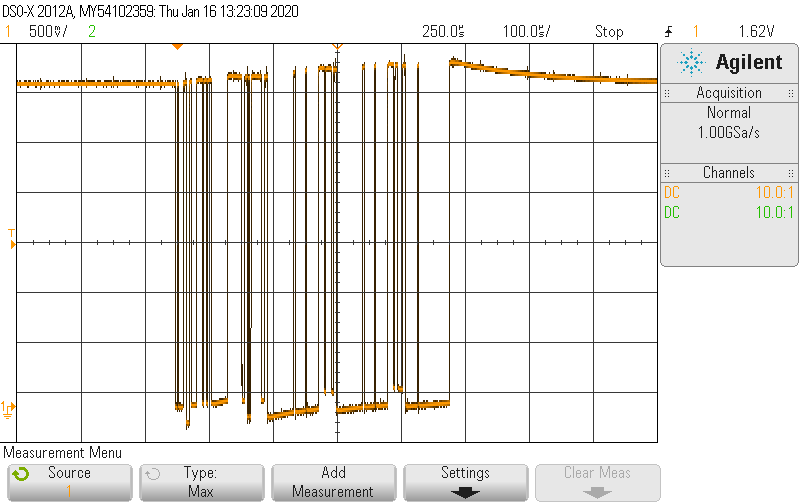
\includegraphics[height=2.60417in]{figs/OpenOCDPollingGood.png}
\caption{OpenOCD periodic poll when it gets a response from the SAM4S.}
\end{figure}

\begin{figure}
\centering
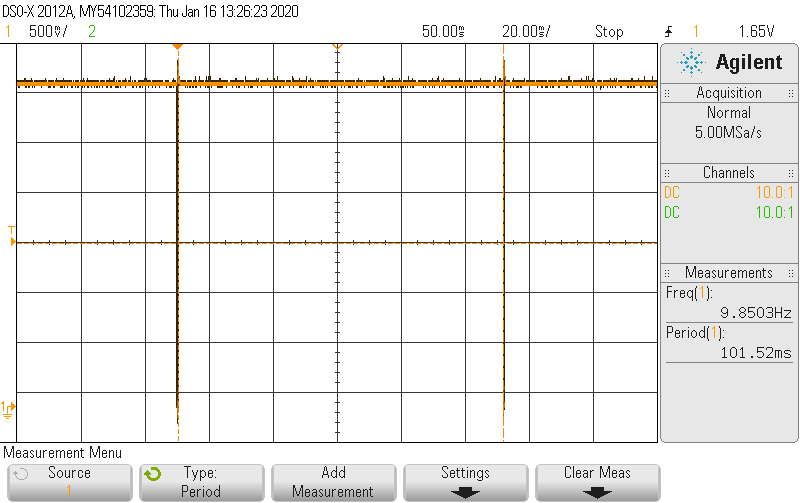
\includegraphics[height=2.60417in]{figs/OpenOCDTimingGood.png}
\caption{OpenOCD polls every 100\,ms while connected.}
\end{figure}

OpenOCD polls less often when it does not get a response. The period
increases to 6300\,ms.

\subsection{Checking the crystal oscillator}
\label{checking-the-crystal-oscillator}

When the SAM4S is first powered up it uses an internal oscillator.
However, when a program is loaded it switches to the main oscillator
that uses the external crystal. If there is a problem with the crystal
oscillator the SAM4S will not run since it has no clock. Moreover,
\program{OpenOCD} will then fail to communicate with the SAM4S.

\begin{figure}
\centering
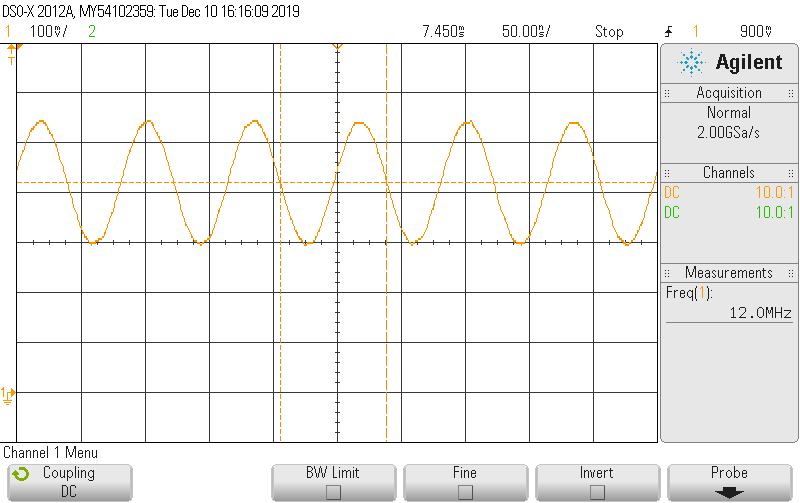
\includegraphics[height=2.60417in]{figs/ClockSignal.png}
\caption{12\,MHz clock sine wave.}
\end{figure}

\mtodo{Add scope picture of CPU clock signals when not working}

\begin{enumerate}
\item
  Connect a scope pin to the XOUT pin. A 12\,MHz sinewave should be
  visible.
\item
  If there is no sinewave:

  \begin{enumerate}
  \item
    Measure the voltage on the VDDPLL pin of the MCU with a scope. This
    should be 1.2 V to power the oscillator.
  \item
    Check the bypass capacitors across the crystal. These should be
    approx. 20 pF.
  \end{enumerate}
\end{enumerate}

\subsection{Checking the clock}
\label{checking-the-clock}

The SAM4s has multiple clock sources:

\begin{enumerate}
\item
  Internal fast RC oscillator (this is selected when the SAM4S is first
  ever used).
\item
  Internal slow RC oscillator (this can be selected to save power).
\item
  Main oscillator using external crystal.
\end{enumerate}

The SAM4S uses a phase-locked-loop (PLL) to multiply the frequency of
the clock source to provide the CPU clock. Sometimes the PLL will run
without a clock source and thus will generate an unexpected frequency.

The clock frequency can be checked by connecting a scope to a peripheral
pin that generates a clock, e.g., PWM, SCK, TXD.

\section{USB serial}
\label{debugging-usb}

USB is a complicated protocol and there are many possibilities why it
does not work.

  \begin{itemize}
  \item
    Check that the termination resistors are 27\,ohms.
    
  \item Check the SAM4S is running at the correct frequency of
    96\,MHz. Check the SAM4S XIN pin with an oscilloscope for a
    12\,MHz sinusoid. Note, the oscillator is not enabled unless a
    program has been loaded and running. If a 12\,MHz signal is not
    found, check the MCU solder connections under a microscope. Also
    check that the VDDPLL pin has 3.3\,V.
  \end{itemize}

  If the USB serial connection drops characters:
  %
 \begin{itemize}
 \item Add a delay before sending data.  This is because the driver
   takes a while to set up the connection after the USB cable is
   plugged in If you try to send some data in this time, the data gets
   stored into a ring buffer for later transmission.  However, the
   ring buffer is not large and once it is filled, the USB serial
   driver will drop characters.
 \end{itemize}

\section{Testing peripherals}
\label{testing-peripherals}

 
\subsection{Motors}
 
\subsection{Debugging PWM}
\label{debugging-pwm}

If PWM does not work:

\begin{enumerate}
\item
  Check the SAM4S pin since not every pin can be a PWM signal
\item
  Check the definition in the configuration file \file{target.h}
\end{enumerate}

If the PWM frequency is wrong:

\begin{enumerate}
\item
  Check the clock frequency, see \hyperref[checking-the-clock]{Checking the clock}.
\item
  Check your program.
\end{enumerate}

If the PWM duty is wrong:

\begin{enumerate}
\item
  Check your program. The duty is specified as an integer in parts per
  thousand. (e.g. 1000 = 100\% duty cycle; 50 = 5\% duty cycle)
\end{enumerate}

\begin{figure}
\centering
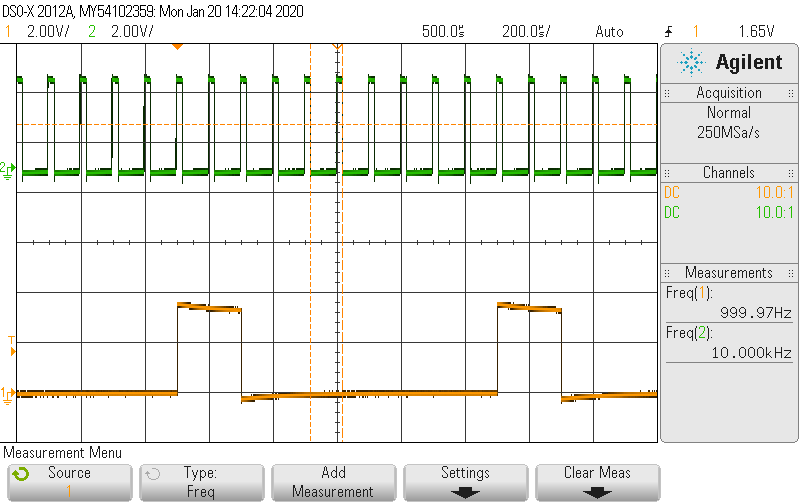
\includegraphics[height=2.60417in]{figs/PWM_2.png}
\caption{Two PWM signals at 1\,kHz and 10\,kHz.}
\end{figure}


\subsubsection{Testing the H-bridge}
\label{testing-the-h-bridge}

\mtodo{TODO}


\subsection{IMU}
\label{imu}

\subsection{Debugging I2C}
\label{debugging-i2c}

\begin{enumerate}
\item
  I2C/TWI requires external pull-up resistors for the clock (TCK) and
  data (TDA) signals.
\item
  TWI channel 1 (TWI1) uses \pin{PB4} and \pin{PB5}. However, these are configured
  on boot as JTAG pins. You can disable this, see
  \hyperref[disabling-jtag-pins]{disabling JTAG pins}.
\end{enumerate}

\mtodo{Add scope picture of I2C signals}

\mtodo{Add scope picture of I2C signals with no acknowledge}

\subsection{NRF24L01+ radio}
\label{nrf24l01-radio}

For the radio to work you need:

\begin{enumerate}
\item
  A working SPI interface.
\item
  The correct channel and address.
\item
  A well filtered power supply for the radio.
\item
  A channel with little interference (note, some channels are shared
  with WiFi and Bluetooth and may be less reliable).
\end{enumerate}

If nothing works, check:

\begin{enumerate}
\item
  For transmission the CE pin should be low; for reception the CE pin
  should be high.
\item
  Check that the SPI clock SCK, MOSI, and MISO signals are driven when
  the radio is configured (note, the MISO signal is tristate when CS is
  high).
\item
  Check that the SPI CS signal is driven low for each transmitted byte.
\end{enumerate}

If the radio transmits but not receives, check:

\begin{enumerate}
\item
  The IRQ pin is driven low (this indicates that a packet has been
  received).
\item
  The power supply. The radio requires a well filtered power supply
  otherwise the range will be limited on reception. Preferably, the
  device should have its own 3V3 regulator with a low-pass RC filter
  comprised of a series resistor and large capacitor (say 22\,$\mu$F) or a
  low-pass LC filter made with a ferrite bead and capacitor.
\end{enumerate}

\textbf{Note}, by default the radio waits for an auto-acknowledgement
from the receiver device. This acknowledgement is performed in hardware.
If no acknowledgement is received, it retries for up to 15 times. The
auto-acknowledgement and number of retries can be configured in
software.

\subsubsection{Checking the radio power supply}
\label{checking-the-radio-power-supply}

\mtodo{Add scope picture of expected radio power supply voltage}

\subsubsection{Debugging SPI}
\label{debugging-spi}

Check:
%
\begin{enumerate}
\item The device chip select signal is driven low.
\item The \code{SCK} signal toggles while the chip select is low.
\item The \code{MOSI} signal does something while the chip select is low.
\end{enumerate}
%
The \code{MISO} signal is usually tri-state and is driven by the
device when the chip select is low.

The SPI standard is rather loose and there are four modes to confuse
the unwary; these are due to two clock polarity modes and two clock
phase modes.  When using the wrong mode, the read data can be
bit-shifted or unreliable.

\mtodo{Add scope picture of SPI signals}

\section{Other problems}
\label{faq}

\begin{itemize}
\item
  \emph{\program{OpenOCD} does not run}. The most common problem is that the
  USB permissions are not correct.
\item
  \emph{A program does not correctly build after a file has been
  changed}. Every now and then the file timestamps are incorrect (this
  is a common problem with network drives due to a skew in the clocks)
  and make will not correctly rebuild a file. Running \textbf{make
  clean} will remove the existing dependency and object files so you can
  start afresh.
\item
  \emph{A program hangs.} This can be observed by an LED no longer
  flashing. There are a number of reasons:

  \begin{itemize}
  \item
    The program is stuck in an infinite loop. Note, an embedded system
    should only have an infinite loop for the main loop; all other loops
    should have a timeout condition.
  \item
    The program has crashed trying to access invalid memory. Usually
    this is due to buffer overflow or dereferencing uninitialised
    pointers (say by not calling \code{radio\_init}). Try running
    'make debug'. This will start the
    \protect\hyperref[debugging]{debugger} and attach to your MCU. If
    the debugger says that your program has stopped in
    '\_hardfault\_handler', then your program is likely to have accessed
    invalid memory. Use the 'bt' command to print a stack trace to see
    how your program went astray.
  \end{itemize}
\item
  \emph{The output of the 3V3 regulator works fine when powered from USB
  but gives 6 V when powered from a 7.2 V battery}. Check that the 7.2 V
  is not connected directly to a SAM4S pin (say for battery monitoring)
  since this will cause an ESD protection diode inside the SAM4S to
  conduct.
\end{itemize}



\appendix
\chapter{OpenOCD}

The Open On-Chip Debugger (OpenOCD) is an open-source on-chip
debugging, in-system programming, and boundary-scan testing tool. It
is able to communicate with various ARM and MIPS microprocessors via
\wikiref{JTAG}{JTAG} or \wikiref{SWD}{SWD}. It works with a number of different
\wikiref{JTAG}{JTAG} or \wikiref{SWD}{SWD} interfaces/programmers. User
interaction can be achieved via telnet or the GNU debugger (GDB).

\section{Configuration files}
\label{configuration-files}

OpenOCD needs a \wikiref{OpenOCD_configuration}{configuration file} to
specify the interface (USB or parallel port) and the target system.
Unfortunately, these change with every new release of OpenOCD.

\section{Running OpenOCD}
\label{running-openocd}

OpenOCD runs as a daemon program in the background and can be controlled
from other programs using TCP/IP sockets. This means that you can
remotely debug from another computer. The socket ports it uses are
specified in the \wikiref{OpenOCD_configuration}{OpenOCD configuration}
file supplied when it starts. By default, OpenOCD uses port 3333 for
\wikiref{GDB}{GDB} and port 4444 for general interaction using Telnet.

\subsection{Communicating with OpenOCD using telnet}
\label{communicating-with-openocd-using-telnet}

If OpenOCD is running, commands can be sent to it using telnet. For
example,

\begin{minted}{bash}
$ telnet localhost:4444
> monitor flash info 0
\end{minted}

\subsection{Communicating with OpenOCD using GDB}
\label{communicating-with-openocd-using-gdb}

If OpenOCD is running, commands can be set to it with
\wikiref{GDB}{GDB}. There are two steps: connecting to OpenOCD with
the target remote command, and then sending a command with the GDB
monitor command. For example,

\begin{minted}{bash}
$ gdb
(gdb) target remote localhost:3333
(gdb) monitor flash info 0
\end{minted}

\section{OpenOCD commands}
\label{openocd-commands}

All the gory OpenOCD details can be found in the
\wikiref{Media:openocd.pdf}{OpenOCD manual}. If you are getting strange
errors see \wikiref{OpenOCD_errors}{OpenOCD errors}.

\section{Flash programming}
\label{flash-programming}

OpenOCD can program the flash program memory from a binary file.

\section{FTDI support}
\label{ftdi-support}

Many \wikiref{JTAG_interface}{JTAG interfaces} use chips made by Future
Technology Devices International (FTDI) to translate between the USB and
JTAG protocols. FTDI provide a library to communicate with these
devices; however, this is not open-source and hence cannot be
distributed. There is an open-source equivalent,
\href{http://freshmeat.net/projects/libftdi/}{libftdi}, which in turn
uses the open-source libusb. This can be temperamental to get working on
a Windows system.

\section{Getting OpenOCD}
\label{getting-openocd}

The developers of OpenOCD release source packages (and provide
subversion access) but do not provide official builds for any
operating system. However, there are various sites which provide
prebuilt versions of OpenOCD.

\subsection{Windows}
\label{windows}

Windows installers for release versions of OpenOCD can be found
\href{http://www.freddiechopin.info/index.php/en/download/category/4-openocd}{here}.
Some development versions can be found
\href{http://www.freddiechopin.info/index.php/en/download/category/10-openocd-dev}{here}.
Unless you need a feature not present in the release version, avoid
getting the development versions as they can be less stable.

Alternatively, the
\href{http://www.siwawi.arubi.uni-kl.de/avr_projects/arm_projects/}{WinARM}
toolchain contains a version of OpenOCD, albeit one that appears (from
the description on the project page) to be out of date. It is also
possible to build your own copy of OpenOCD using either
\href{http://www.mingw.org/}{MinGW} or
\href{http://www.cygwin.com/}{Cygwin}; instructions for this are posted
in various places online.

Realistically, it's probably easier to set up a virtual machine with
Linux and use that instead.

\subsection{Linux}
\label{linux}

Many recent distributions of Linux have OpenOCD in their software
repositories. However, this is often out of date and (in some cases)
buggy. In this case it is straightforward to
\wikiref{Building_OpenOCD_under_Linux}{build the latest version}.

\subsection{Mac OSX}
\label{mac-osx}

The easiest way to install OpenOCD on Mac OSX is to use
\href{http://brew.sh/}{Homebrew}. If you wish to use JTAG with an
adaptor based on a FTDI chip (for example, the UCECE USB to JTAG
adaptor or a Bus Blaster), make sure you include libftdi support by
installing with the command:
%
\begin{minted}{bash}
$ brew install openocd --enable-ft2232_libftdi
\end{minted}

\section{Errors}
\label{errors}

See \wikiref{OpenOCD_errors}{OpenOCD errors}.


\end{document}
